\documentclass{beamer}
%\usepackage[usenames,dvipsnames]{xcolor}

\usepackage{_defsAndPackages675notation}
\usepackage{_defsAndPackages675beamer}

\begin{document}

\title{\alg{Introduction, Notation, and Overview}}
\subtitle{\classTitle}
%\author{\alg{Darren Homrighausen, PhD}}
%\institute{\classTitle}
\date{}



\begin{frame}
\maketitle
%\titlepage
%\begin{figure}[h!]
%  \centering
%  \includegraphics[width=1in]{../figures/CSU_logo2.eps}
%\end{figure}
%
\organization
%
\end{frame}



\begin{frame}

\begin{figure}[h!]
  \centering
  \includegraphics[width=2.5in]{../figures/data_mining.pdf}
\end{figure}
\vsp

\smallCapGreen{Statistical learning and data mining} is about..
\vsp
 
\begin{itemize} 
\item discovering structure in data
\item making predictions about unknown quantities
\end{itemize}


\end{frame}

\begin{frame}
\frametitle{Class Overview}

Practically speaking, this means we seek to:
\vsp

\begin{itemize}
\item 
find relationships between a group of \alg{explanatory} and \alg{response} variables that
provides good predictive performance
\item reduce the \alo{size} of the group of variables for scientific, statistical, or computational
purposes
\end{itemize}
\vsp

and, perhaps most importantly..

\vsp
Knowing the techniques, how they work, when they apply, and how to implement them

\end{frame}

\begin{frame}
\frametitle{Class Outline}
Over the next semester we will address:

\begin{enumerate}
\item High dimensional classification and regression
\item Nonparametric methods
\item Clustering
\item Graphical models
\end{enumerate}

\vsp

This course will emphasize methods and applications.  However, theory will be presented to illustrate 
some important points/techniques.

\end{frame}

\begin{frame}
\frametitle{References:}
\alo{Main references:}
\begin{itemize}
\item {\it The Elements of Statistical Learning} {\scriptsize Hastie, Tibshirani, Friedman}
\item {\it Weak Convergence and Empirical Processes} {\scriptsize Van der Vaart, Wellner}
\end{itemize}

\vsp
\alo{Secondary references:}
\begin{itemize}
\item {\it Statistics for High-Dimensional Data} {\scriptsize B\"uhlmann, Van de Geer}
\item {\it Generic Chaining} {\scriptsize Talagrand}
\item {\it Introduction to Nonparametric Regression} {\scriptsize Tsybakov}
\item {\it Convex Optimization} {\scriptsize Boyd, Vandenberghe}
\end{itemize}

\end{frame}

\transitionSlide{High level overview}

\begin{frame}
\frametitle{So many possibilities}
There are many ways this course can go:

\vsp
\begin{enumerate}
\item \smallCapGreen{Theory:} How to prove results about methods and understand statistical/quantitative papers
\item \smallCapGreen{Methodology:} Discuss the motivation and `inner workings'
\item \smallCapGreen{Applications:} Go over implementation, use of software, data problems
\item \smallCapGreen{Computation:} Go through algorithms, parallelization, data structures...
\end{enumerate}
\vsp

\pause
\smallCapGreen{Task:} Assign a percent to each category representing your interests.
\end{frame}

\transitionSlide{Statistical learning terminology}

\begin{frame}
\frametitle{Introduction}
\alg{Statistical Machine Learning  (SML)} is statistics with a focus on \alo{prediction}, \alo{scalability}, and 
\alo{high dimensional problems}
\vsp

\alg{Regression:} predict $Y \in \mathbb{R}$ from covariates or \alg{features} $X$

\vsp
\alg{Classification:} predict $Y \in \{0,1\}$ from covariates or \alg{features} $X$

\vsp

\alg{Finding structure:} 
\begin{itemize}
\item Finding groups or \alg{clusters} in the data
\item Dimension reduction
\item Graphical models (conditional independence structure)
\end{itemize}
%\script{Note that many SML procedures have already been covered in the program
%under a slightly different guise, including Dr. Cooley's multivariate
%class, concurrent with this class}
\vsp

\end{frame}

\begin{frame}
\begin{center}
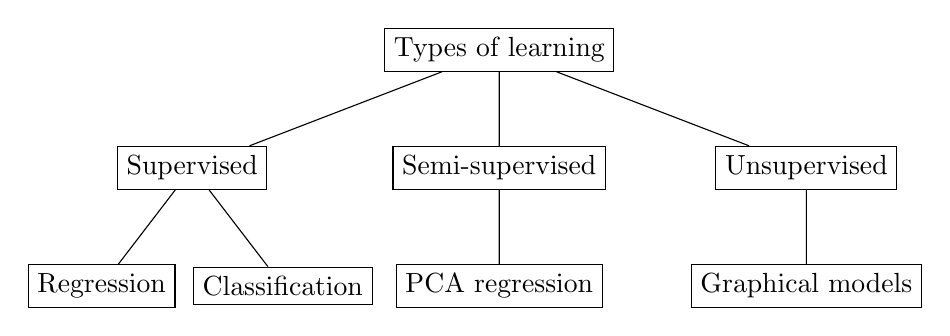
\begin{tikzpicture}
    \tikzstyle{every node}=[rectangle,draw]
    \tikzstyle{level 1}=[sibling distance=39mm] 
    \tikzstyle{level 2}=[sibling distance=23mm]     
    \node {\smallCapGreen{Types of learning}}
        child { node {\alr{Supervised} }
            child { node {\alr{Regression}}}
            child { node {\alr{Classification}} }
        }
        child { node {\alr{Semi-supervised}}           
            child { node {\alb{PCA} \alr{regression}}} 
        }
        child { node {\alb{Unsupervised}}
            child { node {\alb{Graphical models}} }
         }
         ;
\end{tikzpicture}
\end{center}
\vsp

Some comments:
\begin{itemize}
\item[] \alr{Comparing to the response $Y$ gives a natural notion of prediction accuracy}
\item[] \alb{Much more heuristic, unclear what a good solution would be.  We'll return to this later in the semester.}
\end{itemize}
\end{frame}

\begin{frame}
\frametitle{Three main themes}
\alb{\large{Convexity}}

\vsp
Convex problems can be solved efficiently.  If necessary, we try to approximate nonconvex problems with convex ones

\vvsp
\alb{\large{Sparsity}}

\vsp
Many interesting problems are high dimensional 

\script{the number of covariates, $p$, is large compared to the number
of observations, $n$}


\vvsp
\alb{\large{Assumptions}}

\vsp
What assumptions do you need to make to motivate the method or guarantee some property? 
\end{frame}

\transitionSlide{Supervised Methods
\\
\script{We will return to unsupervised methods later in the class}
}

\begin{frame}
\frametitle{The set-up}

We observe $n$ pairs of data $(X_1^{\top},Y_1)^{\top},\ldots,(X_n^{\top},Y_n)^{\top}$

\vsp

Let\footnote{These transposes get tiredsome.  We'll get a bit sloppy and drop them selectively in what follows.}  
$Z_i^{\top} = (X_i^{\top},Y_i) \in \mathbb{R}^{p}\times\mathbb{R}$

\vsp
We'll refer to the \alg{training data} as $\data = \{ Z_1, \ldots, Z_n\}$

\vsp
Call $Y_i$ the \alg{response}, while $X_i$ is the \alg{feature} or \alg{covariate} (vector)

\vvsp
\emphasis{7cm}{Example:}{$Y_i$ is whether a threat is detected in an image and the $X_{ij}$ is the
value at the $j^{th}$ pixel of an image ($p$ might be $1024^2 = 1048576$)}

\end{frame}


\begin{frame}
\frametitle{The set-up}
We use the \alg{training data} $\data$ to \alg{train} an algorithm, producing a 
function $\hat f: \mathbb{R}^p \rightarrow \R$

\vsp
\smallCapGreen{Goal:} Given a new $X \in \R^p$, we want to form 
\alo{predictions}
\[
\hat{f}(X) = \hat{Y}(X,\data) = \hat{Y}
\]

Such that $\hat{Y}$ is a \alo{good} prediction of $Y$, the unobserved response

\end{frame}

\transitionSlide{Risk, Bayes, bias, variance, and approximation}

\begin{frame}
\frametitle{Loss functions and risk}
What determines good?
\vsp

Define a function\footnote{This is the loss for \alo{prediction}.  Other tasks may
have a different domain.} $\ell:\R\times\R \rightarrow \R$ such that smaller values of $\ell$ indicate \alo{better} performance

\vsp 
Two important examples:
\begin{itemize}
\item $\ell(\hat{f}(X),Y) = (\hat{f}(X) - Y)^2$ (regression, square-error)
\item $\ell(\hat{f}(X),Y) = \mathbf{1}(\hat{f}(X) \neq Y)$ (classification, 0-1)
\end{itemize}

\vsp

These expressions are both \alo{random variables}.  This leads us to define the (prediction or generalization) \alg{risk} of a procedure $\hat f$ to be
\[
R(\hat f) = \E\ell(\hat{f}(X),Y) = \P\ell(\hat{f}(X),Y) = \P\ell_{\hat{f}}= \int \ell(\hat{f}(X),Y) d\P,
\]
where $\P$ is the measure induced by $Z = (X,Y)$.
\vsp

\end{frame}


\begin{frame}
\frametitle{Risky (and lossy) business}
The theoretical basis for prediction/estimation is rooted in
\alg{Statistical Decision Theory}.

\vsp
Any distance function\footnote{Or, for that matter, topology} could serve for the loss
function $\ell$

\vsp
We can write the risk as
\[
R(f) = \E \ell(f(X),Y) = \E_X \E_{Y|X} \ell(f(X),Y)
\]
\script{The \alo{tower property} of conditional expectation}

\vsp
The measureable function $f_*$ such that this pointwise relation holds:
\[
f_*(x) = \argmin_c \E_{Y|X=x} \ell(c,Y)
\]
is known as the \alg{Bayes rule} with respect to the loss function $\ell$.
\end{frame}

\begin{frame}
\frametitle{An example: Squared-error loss}
If the function $\ell(f(X),Y) = (f(X) - Y)^2$, then
\[
f_*(x) = \E [Y | X= x].
\]
This is known as the \alg{regression function}; that is, the conditional expectation
of $Y$ given $X$.

\script{This is the Bayes rule with respect to the squared error loss function.}
\vsp

\vsp
This gives rise to the model
\[
Y = f_*(X) + \epsilon
\]
where $\epsilon$ is some mean zero fluctuation

\end{frame}


\begin{frame}
\frametitle{An example: Zero-one loss}
Instead, let $Y \in \mathcal{G} = \{1,\ldots, G\}$ 
\vsp

As $Y$ takes only a few values, \alo{zero-one} prediction risk is natural
  \[
  \ell(f(X),Y) = \mathbf{1}(Y\neq f(X)) \; \Longrightarrow \; R(f) = \E[\ell(f(X),Y)] = ?
  \]
  
\script{? $=$ \textcolor<2>{black}{\textcolor<1>{white}{$\P(f(X) \neq Y)$}}}

\vsp
%\alg{label} or \alg{classify} 
\smallCapGreen{Goal:} Find an $f$ such that $f(X) = Y$ as often
as possible

\vsp
Under this loss, we have
\[
f_*(X) = \argmin_{g \in \mathcal{G}} \left[ 1 - \P(Y = g | X)\right]  = \argmax_{g \in \mathcal{G}} \P(Y = g | X )
\]

\script{\smallCapGreen{Interpretation:} The Bayes rule for classification with this loss
is to pick the class that maximizes the conditional probability of $Y$ being that class}
\end{frame}



\begin{frame}
\frametitle{Training error and risk estimation}
Of course, we don't know $\P$...

\vsp
We need to estimate it!
\vsp

Perhaps the most intuitive estimate of the measure $\P$ is
\[
\hat{\P} = \frac{1}{n}\sum_{i=1}^n \delta_{Z_i},
\]
where 
$\delta_{x}$ is a (probability) measure that puts mass 1 at $x$.
\vsp

This is known as the \alg{empirical measure} of $\data$
\vsp

Just like $\P f(X) = \int f(X) d \P$, we can write
\[
\hat{\P} f(X) = \int f(X) d \hat{\P} = \frac{1}{n}\sum_{i=1}^n f(Z_i).
\]
\end{frame}

\begin{frame}
\frametitle{Example: Maximum likelihood estimation}
Suppose that we are interested in estimating a parameter vector $\mu$

\vsp
We specify a \alo{likelihood} $L_\mu(Z)$, such as by stating $Z \sim N(\mu,\Sigma) \in \R^p$ and writing
\[
L_\mu(Z) = (2\pi)^{-n/2} |\Sigma|^{-1/2} e^{- (Z - \mu)^{\top} \Sigma^{-1} (Z- \mu)/2}. 
\]

Define $\ell_\mu = \log L_\mu$.  Then the maximum likelihood estimator is
\[
\argmax_\mu \hat \P \ell_\mu
\]

\end{frame}
%
%\begin{frame}
%\frametitle{Decomposition}
%Suppose $\F$ is a function class.  If we write
%\[
%\hat{f}_*(x) = \argmin_{f \in \F} \E_{Y|X=x} (f(x) - Y)^2,
%\]
%then $\hat{f}_*$ is best possible element of (our model) $\F$.
%
%\vsp
%We can break the Bayes risk into four components
%\begin{align*}
%\E(f(X) - Y)^2 
%& = 
%\E(f(X) - \hat{f}_*(X) + \hat{f}_*(X) - f_*(X) + f_*(X) - Y)^2 
%\end{align*}
%\end{frame}
%

\transitionSlide{Linear Algebra}


\begin{frame}
\frametitle{Background}
\begin{itemize}
\item We will write \alg{vectors} as 
\[
z = 
\begin{bmatrix}
z_1\\
z_2\\ 
\vdots \\
z_n
\end{bmatrix}
\]
We write this as $z \in \mathbb{R}^n$, which is ``z is a member of ar-en.''
\item We commonly will need to ``turn'' the vector, which we write as
\[
z^{\top}
=
\begin{bmatrix}
z_1 & z_2 & \ldots & z_n
\end{bmatrix}
\]
\end{itemize}
\end{frame}

\begin{frame}
\frametitle{Necessary Background: Notation}

We will concatenate the \alo{covariates} or \alo{features} into the \alg{design} or \alg{feature} matrix $\X$,
where

\begin{align*}
\X 
& = 
\begin{bmatrix}
x_1 &  x_2 & \cdots & x_p
\end{bmatrix} 
%& =
%\begin{bmatrix}
%x_{11} & x_{21} & \ldots & x_{1p} \\
%x_{12} & x_{22} & \ldots & x_{2p} \\
%&&\vdots & \\
%x_{1n} & x_{n2} & \ldots & x_{np} \\
%\end{bmatrix} \\ 
= 
\begin{bmatrix}
X_1^{\top} \\
 X_2 ^{\top}\\
 \vdots \\
  X_n^{\top}
\end{bmatrix}
\in
\R^{n \times p}
\end{align*}
%We will also write the $(i,j)^{th}$ entry of a matrix $\X$ as $\X_{ij}$ and say $\X \in \mathbb{R}^{n \times p}$.
%
%\vsp
%As much as possible
%\begin{itemize}
%\item \alg{Lower case} Roman letters will be columns
%\item \alg{Upper case} Roman letters will be rows
%\end{itemize}

\vsp
\smallCapGreen{In words:} The covariates (columns) will be lower case letters
and the observations (rows) will be upper case letters

\vsp
\script{It appears as though the book goes back and forth between capital and lower case for various quantities}
\end{frame}

\begin{frame}
\frametitle{Norms}
We will need to measure the \alo{size} of vectors

\vsp
The most common one is the one we use every day (implictly): \alg{Euclidean distance}\footnote{Think:
the Pythagorean theorem.}
\[
|| \x ||_2 = \sqrt{\sum_{k=1}^p x_k^2}
\]

\vsp
Additionally, we will need the \alg{Manhattan distance}

\[
|| \x ||_1 = \sum_{k=1}^p |x_k|
\]

\vsp
In general, the \alg{$\ell^r$ norm} is:
\[
|| \x ||_r = \left(\sum_{k=1}^p |x_k|^r\right)^{1/r}
\]


\end{frame}


\transitionSlide{Singular Value Decomposition (SVD)}

\begin{frame}
\frametitle{Singular value decomposition (SVD)}

A huge amount of statistics depends on (numerical) linear algebra concepts

\vsp
Many, many topics in (numerical) linear algebra are implicitly motivated by
the \alg{singular value decomposition (SVD)} 

\vsp
Some examples are:

\begin{itemize}
\item Multiple regression
\item Penalized least squares
\item Principal components analysis
\item Discriminant analysis
\end{itemize}

\end{frame}


\begin{frame}
\frametitle{SVD}

The SVD is a generalization of the eigenvector decomposition

\vsp
Instead of
\[
\X = U D \alr{U}^{\top} \longleftarrow \textrm{eigenvector decomposition}
\]
we get
\[
\X = U D \alr{V}^{\top} \longleftarrow \textrm{singular value decomposition}
\]
This change makes the (unique) SVD always exist

\script{As opposed to the eigenvector decomposition which only exists sometimes}
\end{frame}



\begin{frame}
\frametitle{Singular value decomposition (SVD)}
It turns out we can think of matrix multiplication in terms of circles and ellipsoids

\vsp
Take a matrix $\X$ and let's look at the set of vectors 
\[
B = \{ \beta: ||\beta||_2 \leq 1\}
\]

\vsp
This is a circle!
\begin{center}
\includegraphics[width=1.55in]{../figures/intro_circle.pdf}
\end{center}
\end{frame}

\begin{frame}
\frametitle{Singular value decomposition (SVD)}
What happens when we multiply vectors in this circle by  $\X$?

\vsp

Let 
\[
\X = 
\begin{bmatrix}
2.0 & 0.5 \\
1.5 & 3.0 
\end{bmatrix}
\textrm{ and } 
\X \beta
=
\begin{bmatrix}
2\beta_1 + 0.5\beta_2 \\
1.5\beta_1 +3\beta_2 
\end{bmatrix}
\]
\begin{columns}[T]
    \begin{column}{.38\textwidth}
\includegraphics[width=1.75in]{../figures/intro_circle.pdf}
\end{column}
    \begin{column}{.05\textwidth}
    \vsp
    
    \vsp
    
    \vsp
    
    \vsp
    
    \vsp
\[
\stackrel{\X}{\longrightarrow}
\]
\end{column}
    \begin{column}{.37\textwidth}
\includegraphics[width=1.75in]{../figures/intro_ellipse.pdf}
\end{column}
\end{columns}
\end{frame}

\begin{frame}
\frametitle{Singular value decomposition (SVD)}

\begin{columns}[T]
    \begin{column}{.38\textwidth}
\includegraphics[width=1.75in]{../figures/intro_circle.pdf}
\end{column}
    \begin{column}{.05\textwidth}
    \vsp
    
    \vsp
    
    \vsp
    
    \vsp
    
    \vsp
\[
\stackrel{\X}{\longrightarrow}
\]
\end{column}
    \begin{column}{.37\textwidth}
\includegraphics[width=1.75in]{../figures/intro_ellipse.pdf}
\end{column}
\end{columns}

What happened?

\vsp
\begin{enumerate}
\item The coodinate axis gets \alo{rotated}
\item The new axis gets \alo{elongated} (making an \alg{ellipse})
\item This ellipse gets \alo{rotated}
\end{enumerate}

\vsp
Let's break this down into parts...
\end{frame}

\begin{frame}
\frametitle{Singular value decomposition (SVD)}

\includegraphics<1>[width=1.75in]{../figures/intro_circleAnnotated.pdf}
\includegraphics<1>[width=1.75in]{../figures/intro_circleAnnotatedV.pdf}

\includegraphics<2>[width=1.75in]{../figures/intro_circleAnnotatedV.pdf}
\includegraphics<2>[width=1.75in]{../figures/intro_circleAnnotatedVD.pdf}

\includegraphics<3>[width=1.75in]{../figures/intro_circleAnnotatedVD.pdf}
\includegraphics<3>[width=1.75in]{../figures/intro_ellipseAnnotated.pdf}

\vsp
\begin{enumerate}
\item<1->[1.] The coordinate axis gets \alo{rotated}
\item<2->[2.] The new axis gets \alo{elongated} (making an \alg{ellipse})
\item<3->[3.] This ellipse gets \alo{rotated}
\end{enumerate}

\end{frame}


\begin{frame}% Recap
\frametitle{Rotation and Elongation}

\vsp
\emphasis{8.5cm}{Rotations:}{These can be thought of as just \alo{reparameterizing} the coordinate axis.  This means 
that they don't change the geometry.  As the original coordinate axis was \alg{orthogonal} (that is;
perpendicular), the new coordinates must be as well.  }

\vsp Let $\v_1, \v_2$ be two \alg{normalized, orthogonal} vectors.  This means that:
\[
\v_1^{\top} \v_2 = 0 \quad \textrm{and} \quad \v_1^{\top}\v_1 = \v_2^{\top}\v_2 = 1
\]

In matrix notation, if we create $V$ as a matrix with normalized, orthogonal vectors as columns, then:
\[
V^{\top} V = 
\begin{bmatrix}
1 & 0 & 0 & \ldots & 0 \\
0 & 1 & 0 & \ldots & 0 \\
&& \vdots && \\
0 & 0 & 0 & \ldots & 1 \\
\end{bmatrix}
=
I
\]
Here, $I$ is the \alg{ identity matrix}.
\end{frame}

\begin{frame}% Recap
\frametitle{Rotation and Elongation}

\vsp
\emphasis{8.5cm}{Elongation:}{These can be thought of as \alo{stretching} vectors along the
current coordinate axis.  This means 
that they \textbf{do} change the geometry by distorting distances. These are given by multiplication
by diagonal matrices.}

\vsp
All diagonal matrices have the form:
\[
D
=
\begin{bmatrix}
d_1 & 0 & 0 & \ldots & 0 \\
0 & d_2 & 0 & \ldots & 0 \\
&& \vdots && \\
0 & 0 & 0 & \ldots & d_p \\
\end{bmatrix}
\]
\end{frame}

\begin{frame}
\frametitle{Singular value decomposition (SVD)}
Using this intuition, for any matrix $\X$ it is possible to write its \alg{SVD}:
\[
\X = U D V^{\top}
\]
where
\begin{itemize}
\item $U$ and $V$ are orthogonal (think: rotations)
\item $D$ is diagonal (think: elongation)
\item The diagonal elements of $D$ are ordered as 
\[
d_1 \geq d_2 \geq \ldots \geq d_p \geq 0
\]
\end{itemize}
Many properties of matrices can be `read off' from the SVD.  

\vsp
\emphasis{9cm}{Rank:}{The rank of a matrix answers the question: how many dimensions does the ellipse live in?
In other words, it is the number of columns of the matrix $\X$, not counting the columns that are `redundant'.  

It turns out the rank is exactly the quantity $q$ such that $d_q > 0$ and $d_{q+1} = 0$.}

\end{frame}

\begin{frame}% Recap
\frametitle{Singular value decomposition (SVD)}

\includegraphics<1>[width=1.75in]{../figures/intro_circleAnnotated.pdf}
\includegraphics<1>[width=1.75in]{../figures/intro_circleAnnotatedVtext.pdf}

\includegraphics<2>[width=1.75in]{../figures/intro_circleAnnotatedVtext.pdf}
\includegraphics<2>[width=1.75in]{../figures/intro_circleAnnotatedVDtext.pdf}

\includegraphics<3>[width=1.75in]{../figures/intro_circleAnnotatedVDtext.pdf}
\includegraphics<3>[width=1.75in]{../figures/intro_ellipseAnnotated.pdf}

\vsp
\begin{enumerate}
\item<1->[1.] The coordinate axis gets \alo{rotated} (Multiplication by $V^{\top}$)
\item<2-> The new axis gets \alo{elongated} (Multiplication by $D$)
\item<3-> This ellipse gets \alo{rotated} (Multiplication by $U$)
\end{enumerate}

\end{frame}

\begin{frame}% Recap
\frametitle{Singular value decomposition (SVD)}
\begin{columns}[T]
    \begin{column}{.62\textwidth}
\begin{figure}
\includegraphics[width=1.4in,trim=30 30 30 30]{../figures/intro_circleAnnotated1.pdf}
\includegraphics[width=1.4in,trim=30 30 30 30]{../figures/intro_circleAnnotated2.pdf} \\
\includegraphics[width=1.4in,trim=30 30 30 30]{../figures/intro_ellipseAnnotated1.pdf}
\includegraphics[width=1.4in,trim=30 30 30 30]{../figures/intro_ellipseAnnotated2.pdf} 
\end{figure}
\end{column}
    \begin{column}{.4\textwidth}
    \vsp
    \vsp
    \vsp
    
    Summary:
    \vsp
    
Of all the possible axes of the original circle, the one given by $v_1, v_2$
has the unique property:
\[
\X v_j = d_j u_j
\]
for all $j$.
\vsp

Lastly:

\[
\X = \sum_j d_j u_j v_j^{\top}
\]

 \end{column}
\end{columns}

\end{frame}

\begin{frame}% Recap
\frametitle{Singular value decomposition (SVD)}
Taking this last formulation:
\[
\X = \sum_j d_j u_j v_j^{\top}
\]

we see that matrix multiplication looks like
\[
\X\beta = \sum_j \alb{d_j} u_j \alb{v_j^{\top}\beta} =  \sum_j u_j  \alb{\theta_j}
\]

\vsp
\smallCapGreen{Implication:} Multiplication by $\X$ re-expresses $\beta$ in a new coordinate system,
with coordinates $\theta^{\top} = [\theta_1,\theta_2,\ldots]$
\end{frame}


%\begin{frame}
%\frametitle{An overarching framework}
%We want to 
%\end{frame}

%\begin{frame}
%\frametitle{The SVD and risk}
%Let $\Sigma  = \V \hat\beta$.  Then, as discussed, we must be able to write $\Sigma$ in its SVD
%\[
%\Sigma = V D V^{\top}
%\]
%{\scriptsize (Due to $\Sigma$ being symmetric, the SVD and eigenvalue decompositions are
%the same thing and $U$ is equal to $V$)}
%
%\vsp
%Also, the trace of a matrix is actually equal to the sum of the eigenvalues $D$.
%
%\vsp
%So, 
%\[
%\tr(\V \hat\beta) = \sum_j d_j
%\]
%
%Hence, the difficulty of an estimation problem can be thought of as ``how eccentric is the ellipse generated by the variance matrix?''
%\end{frame}


%\begin{frame}
%\frametitle{An overarching framework}
%\end{frame}
\end{document}
